\chapter{Malicious URL detection}

This chapter focuses on providing a broader context for malicious URL detection (using URL strings only). It begins by defining, in detail, what a URL is and how it is structured. It then describes the types of attacks that attackers can execute using URLs. The next part focuses on what kinds of information can be used to detect the attacks in general, and what kind of information can be used to detect the attacks using only the URL string. The last part then describes, where the model would fit in a real environment.

\section{What Is a URL?}

A URL (RFC 3986~\cite{rfc3986}) (Uniform Resource Locator) defines the address of a resource on the internet. This section provides a detailed overview of the structure of URLs.

A URL consists of multiple components, each serving a specific syntactic and functional role. The general structure of a URL~\cite{rfc3986} is shown in Figure~\ref{fig:url_syntax}, followed by a real-world example with labelled parts in Figure~\ref{fig:url_structure_example}.

\begin{figure}[H]
    \centering
    \wrappedttt{scheme://[user@]host[:port]/path[?query][\#fragment]}
    \caption{General syntax of a URL. The components are shown in square brackets, indicating that they are optional.}
    \label{fig:url_syntax}
\end{figure}

\begin{figure}[H]
    \centering
    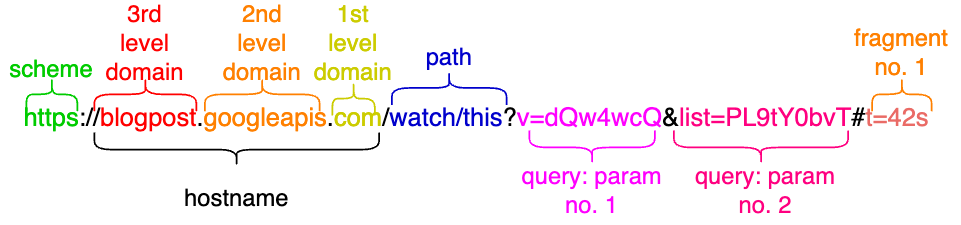
\includegraphics[width=1\textwidth]{images/url_structure_example.png}
    \caption{Example of a URL structure with labelled components}
    \label{fig:url_structure_example}
\end{figure}

Each component of a URL serves a different purpose. Below are the purposes for each section accompanied by a part of a real example depicted in Figure~\ref{fig:url_structure_example}.

\begin{itemize}
    \item \textbf{Scheme:} \wrappedttt{https} indicates the protocol to use. It tells the client (usually a browser) to communicate securely with the server using HTTP over TLS. Common schemes include \wrappedttt{http}, \wrappedttt{https}, \wrappedttt{ftp}, and \wrappedttt{mailto}.
    \item \textbf{User (optional):} Credentials can be embedded in the URL as \wrappedttt{user@host}. For example, \wrappedttt{ftp://admin@ftp.example.com} uses \wrappedttt{admin} as the username. This is uncommon in the modern web and its usage could be a signal of potentially malicious behaviour (this is more explored in the related work section).
    \item \textbf{Hostname:} \wrappedttt{blogpost.googleapis.com} identifies which server should be contacted. It is either an IP address or a DNS-resolvable hostname~\cite{rfc1035}.
    \item \textbf{Path:} \wrappedttt{/watch/this} specifies the location of the resource on the server. Its meaning is interpreted by the server (REST API, file system, etc.). The path is hierarchical and may include multiple segments separated by slashes.
    \item \textbf{Query:} \wrappedttt{?v=dQw4wcQ\&list=PL9tY0bvT} contains URL parameters in key-value pairs. Here, \wrappedttt{v} and \wrappedttt{list} might refer to a video ID and a playlist. Queries allow dynamic interaction with the backend without altering the path.
    \item \textbf{Fragment:} \wrappedttt{\#t=42s} refers to a client-side anchor or setting, such as scrolling to a specific section or timestamp. Fragments are never sent to the server and are interpreted entirely by the browser.
\end{itemize}

\subsection{Hostname}
The hostname component of a URL can take two distinct forms.

The first form is an IP address. IPv4 addresses, as specified in RFC 791~\cite{rfc791}, are represented in dotted-decimal notation, for example \wrappedttt{8.8.8.8}. IPv6 addresses, defined in RFC 8200~\cite{rfc8200}, use a colon-separated hexadecimal format and must be enclosed in square brackets when included in URLs, such as \wrappedttt{[2001:db8::1]}. When an IP address is used as the hostname, DNS resolution is bypassed, and the client connects directly to the specified address.

The second form is a DNS-resolvable domain name, which follows a hierarchical structure. For example, in Figure~\ref{fig:url_structure_example}, the label \wrappedttt{blogpost} is a subdomain of \wrappedttt{googleapis.com}, while \wrappedttt{googleapis} is the second-level domain under the top-level domain \wrappedttt{.com}.

The second-level domain (SLD), such as \wrappedttt{googleapis}, identifies the entity that has registered the domain within a given top-level domain (TLD). Common TLDs include generic domains like \wrappedttt{.com} and \wrappedttt{.org}, as well as country-code TLDs such as \wrappedttt{.cz}. These domains are managed by ICANN (Internet Corporation for Assigned Names and Numbers). The Domain Name System (DNS), as defined in RFC 1035~\cite{rfc1035}, is responsible for resolving domain names to their corresponding IP addresses.

\section{Types of URL-Based Attacks}
\label{sec:types_of_url_attacks}

This section outlines several common types of attacks where the malicious payload or intent is embedded in the URL itself. The selected few that are mentioned here are the most common ones mentioned repeatedly in reports from Webroot 2019 report~\cite{webroot2019} and FBI 2024 report~\cite{fbi2024ic3report} or were present in the datasets used in this thesis.

\begin{itemize}
    \item \textbf{Credential Phishing:} These attacks use deceptive URLs to impersonate legitimate services and trick users into submitting sensitive information like as login credentials or financial details. Attackers often register domains that closely resemble real ones. The key signal that a URL might be leading to a phishing website is that it tries to appear as if it leads to the website it tries to impersonate. According to~\cite{fbi2024ic3report}, a phishing attack in 2024 caused over 70 million USD in losses for US citizens.

    \item \textbf{Drive-by Downloads:} URLs of this type cause the user's browser to automatically download and execute malicious content, typically without user interaction. These may exploit vulnerabilities in the browser or plugins to install malware. They are especially effective if user does not have up-to-date software.

    \item \textbf{Crypto-jacking:} Some URLs lead to pages that execute cryptocurrency mining scripts, consuming the user's computing resources without their consent. This is usually implemented through embedded JavaScript and can be triggered as soon as the page loads.

    \item \textbf{File-less Attacks:} In file-less attacks, the malicious payload is not delivered as a downloadable file, but rather executed directly from memory, often via scripts embedded in the URL itself (e.g., encoded PowerShell, JavaScript, or Bash). These may appear in query strings or path segments and are difficult to detect through traditional signature-based methods.

    \item \textbf{Custom Malicious Content:} Some URLs lead to content that, while not technically malware, is designed to harm users or violate platform policies. This includes links to explicit pornography, scams, illegal downloads, hate content, or violent material. Custom models can be trained to detect these types of URLs, if the organization needs it.
\end{itemize}

\section{Information Usable for Detection}

Multiple types of information can be used to detect whether a given URL is malicious. This thesis proposes a categorization of the information into four groups, similar to the 2017 survey on malicious URL detection~\cite{surveymaliciousfeatures}.

\subsection{Content-based information}
\label{sec:content_based_info}
This information is not at all taken into account for this thesis. It is the information that can be extracted from the content of the page that the URL points to. This includes but is not limited to, the HTML (Hyper-text markup language) content of the page, JavaScript code, and any other resources that are loaded when the page is opened.

Semantic information about the content can be used too. For example, if the content of the page contains content that requires input credentials, it should be more suspicious, because it could be a credential phishing attack. This type of information was usually mined manually by data analysts in the past. However, recent work such as~\cite{koide2025detectingphishingsitesusing} shows that large language models like ChatGPT can process both raw HTML and webpage screenshots to extract high-level semantic cues.

Another type of information that can be extracted from the content of a website is very similar to the content of some high-profile websites. This might indicate that the site is trying to trick users into thinking they are on a some other legitimate website, such as PayPal, while they are in reality going to send their credentials to an attacker. An example of work that tries to leverage this type of information is~\cite{VisualPhishNet}, which uses a triplet Convolutional Neural Network (CNN) to create embeddings of the examined website and compare it against the embeddings of a few legitimate websites.

\subsection{Domain-based metadata}
\label{sec:domain_based_info}
This group consists of every bit of external knowledge about the domain that is present in the URL.

The simplest and most widely used information from this group is the presence of domains on either blocklists or allowlists. Blocklists contain known malicious domains, or IP addresses, which should always be blocked. These are typically maintained by security vendors, threat intelligence services, or community-driven projects like PhishTank~\cite{PhishTank} or OpenPhish~\cite{OpenPhish}. In addition, many organizations maintain their internal blocklists, curated by their Security Operations Center (SOC) teams, based on incidents observed within their networks.

Allowlists, on the other hand, contain trusted URLs that should always be allowed. These can include popular websites, internal company resources, or other trusted domains.

The information about the domain does not have to be absolute -- malicious or benign but can be expressed as a reputation score. Different ranking scores like Google PageRank~\cite{Page1998PageRank} (or similar, that are available publicly) can be used to determine the quality of the domain.

Metadata such as the age of the domain and WHOIS~\cite{whois} registration information has been widely used in prior work~\cite{surveymaliciousfeatures}. For example, domains registered only days before being used are more likely to be malicious~\cite{surveymaliciousfeatures}.

Another type of information also discussed in~\cite{surveymaliciousfeatures}, is whether the domain attempts to mimic a well-known domain. For example, if the domain is \wrappedttt{pay-pal.com} instead of \wrappedttt{paypal.com}, it may be trying to trick users into thinking that they are on the legitimate site. The crucial part here is the inclusion of certain information about the domain the URL tries to impersonate. Should the impersonated domain be a very popular one and hackers might want to target it because of its content (banking, credentials, ...), the URL should be considered more suspicious.

This is not limited to SLDs if the domain is \wrappedttt{paypal.malicious.com}, it may be trying to impersonate the legitimate site as well. Special features, such as Levenshtein distance can be used to determine how similar the domain is to the legitimate one in terms of edit distance.

Another way to determine the similarity try to detect the homoglyph attack, where the attacker uses visually similar characters to trick users into clicking on a malicious link. For example, the letter "o" in the domain \wrappedttt{g00gle.com} is replaced with two zeros.

\subsection{URL-string Based Information}
URL-string-based information refers to any feature that can be extracted directly from the URL string itself, without requiring external lookups or content analysis. This includes structural properties, handcrafted features, specific characters or keywords, semantic hints from query parameters, and common domain name obfuscation patterns.

One example of such information is the presence of the \wrappedttt{@} character. In URL syntax, any part of the string preceding \wrappedttt{@} is treated as user information and ignored during host resolution. For instance, the URL \wrappedttt{http://legitimate.com@malicious.com} appears to reference \wrappedttt{legitimate.com}, but in reality, the browser connects to \wrappedttt{malicious.com}.

Attackers may also exploit excessively long URLs to conceal malicious content. For example, a URL like \wrappedttt{http://example.com/secure/account/update/redirect?next=aHR0cHM6Ly93d3cucGF5cGFsLmNvbS9sb2dpbg==} can seem legitimate at first glance, yet contains a redirect parameter that points to a malicious destination hidden deep within the URL.

Another obfuscation technique in this category known as a homoglyph attack exploits visually similar characters to disguise malicious URLs. Attackers register domains using Unicode characters that closely resemble legitimate ones, tricking users into believing the URL is safe. While users typically see URLs rendered in Unicode, only ASCII characters are transmitted over the network, as specified in RFC 3986~\cite{rfc3986}. Unicode characters are transformed into ASCII-compatible encodings before transmission and later rendered back into a user-friendly form by browsers. Although the visual similarity is lost after encoding, text-based models can still detect such attacks by learning to recognize uncommon character patterns or domain name irregularities that often accompany these manipulations.

Exhaustive research is conducted on this type of information in the related work chapter, as it is the only source of information models trained in this thesis use.

\section{Detection Pipeline}
\label{sec:real_world_pipeline}
This section outlines the overall architecture of a typical malicious URL detection pipeline. Although the primary focus is on large-scale threat intelligence services, it is important to note that optimizing models for size and inference speed can unlock entirely new deployment scenarios (for example deployment directly in the web browser).

In a standard threat intelligence setting, clients submit URLs they wish to verify for potential malicious activity. These requests can easily reach tens of millions per day. To manage such volumes, a multi-stage architecture with progressively more computationally expensive models is used. Each layer attempts to resolve as many URLs as possible before the next step.

\begin{figure}[H]
    \centering
    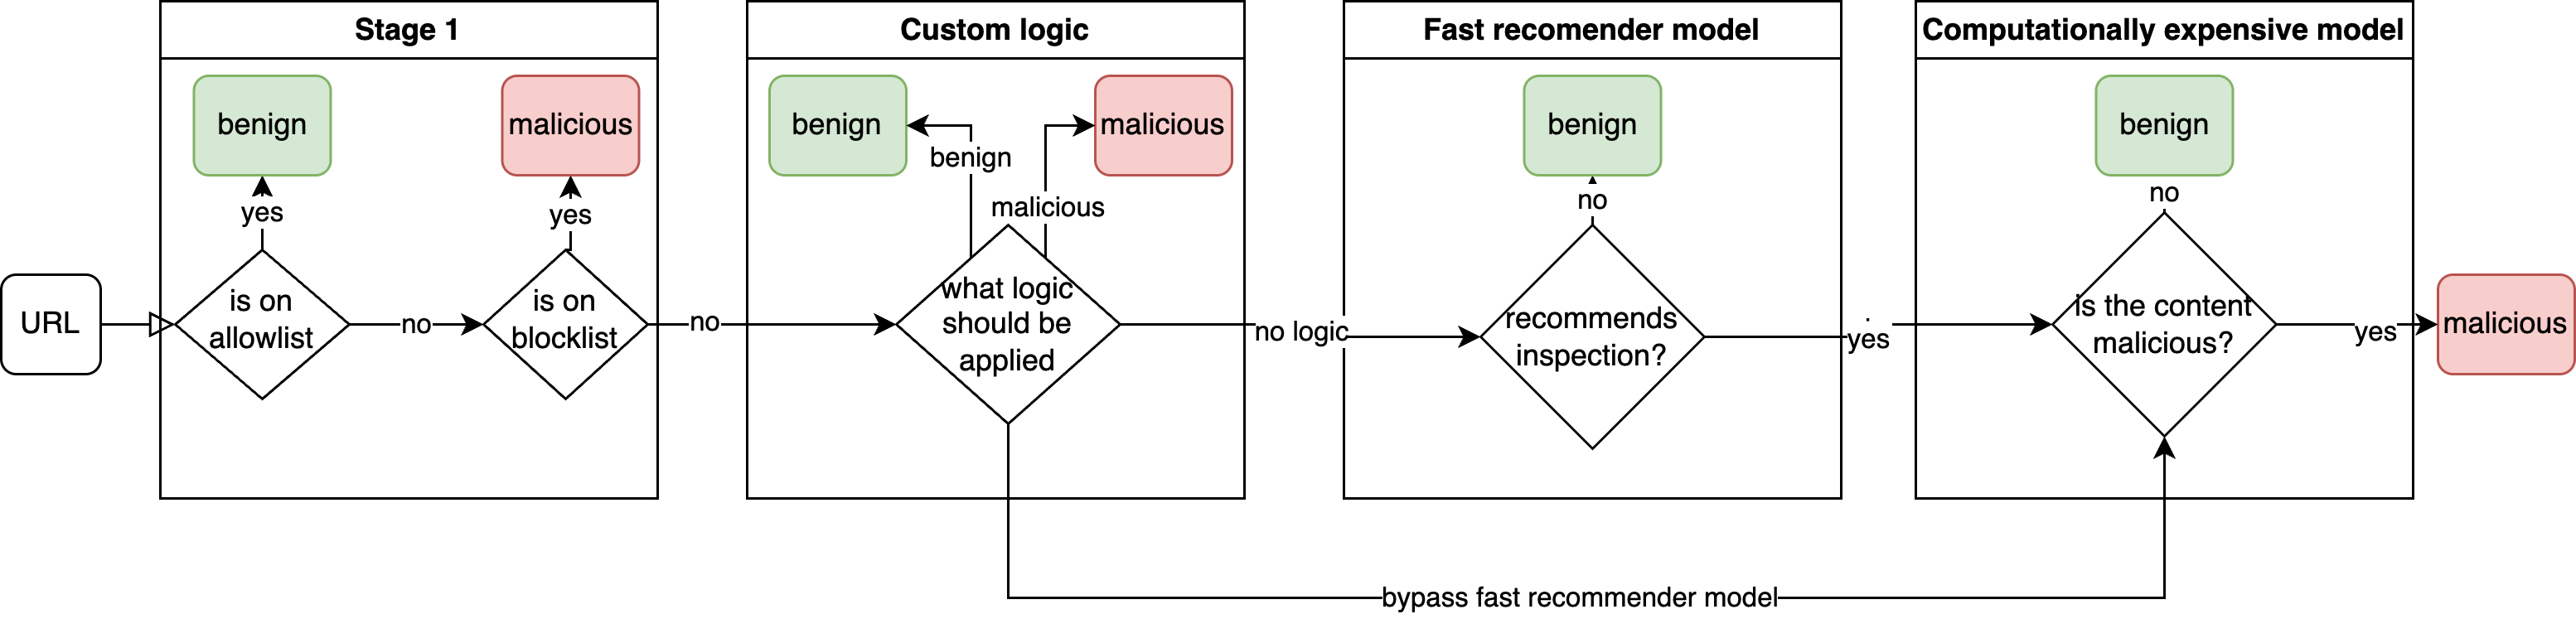
\includegraphics[width=1\textwidth]{images/pipeline_diagram.png}
    \caption{Example of a URL detection pipeline}
    \label{fig:detection_pipeline}
\end{figure}

The typical detection pipeline consists of the following stages, which can be seen in~\ref{fig:detection_pipeline}:
\begin{itemize}
    \item \textbf{Blocklist/Allowlist} -- The first stage filters out URLs based on allowlists of known benign domains and blocklists of known malicious domains. This step quickly discards a significant portion of URLs without further processing. It can be continuously updated based on previous model results.

    \item \textbf{Custom Pre-Filtering} -- Domain-specific rules can be applied in this stage. For example, URL shorteners such as \wrappedttt{bitly.com}~\cite{bitly} generate compact links that redirect to a final destination. These services obscure the actual target URL with a short, seemingly random one, which gives the string-based model no information to classify it correctly. Therefore, a custom logic should automatically flag such URLs for deeper inspection in later pipeline stages.

    \item \textbf{Fast Recommender Model} -- At this stage, a lightweight model processes large volumes of URLs (thousands per second) and flags those that are likely to be malicious. URLs deemed suspicious are passed to the next stage for further analysis, while the rest are discarded.

    \item \textbf{Computationally Expensive Model} -- In this stage, the model uses information from Sections~\ref{sec:content_based_info} about content and from~\ref{sec:domain_based_info} about domains.
\end{itemize}

The model developed in this thesis is intended for the Fast Recommender Stage, where the primary objective is to identify as many malicious URLs as possible, even at the cost of increased false positives -- though this must remain within reasonable limits, as each detection triggers an expensive computational in the next stage.